Zunächst soll auf die zu analysierenden Oberflächen genauer eingegangen werden.
Die deflektometrischen Verfahren wurden explizit für spiegelnde Oberflächen entwickelt.
Doch aus welchem Grund trifft man die Unterscheidung zwischen spiegelnden und nicht-spie\-geln\-den Objekten?
Warum wendet man Verfahren für diffus reflektierende Oberflächen nicht auch für spiegelnde Oberflächen an?
Zur Beantwortung dieser Fragen sollte man die Eigenschaften der Oberflächen genauer betrachten.
Eine diffus reflektierende Oberfläche strahlt die auftreffenden Lichtstrahlen in viele Richtungen ab, wohingegen spekular reflektierende Oberflächen die Lichtstrahlen in eine Richtung reflektieren.
Diffus reflektierende Oberflächen werden als matt oder rau bezeichnet, weil die Lichtstrahlen auf mikroskopischer Ebene auf eine raue Oberfläche treffen.
Spekular reflektierende Oberflächen werden als spiegelnd oder glatt bezeichnet, weil die Lichtstrahlen auf mikroskopischer Ebene auf eine glatte Oberfläche treffen.
Abbildung \ref{tikz:abbGlattUndRau} zeigt diesen Zusammenhang zwischen der mikroskopischen Oberflächenbeschaffenheit und den daraus folgenden Reflexionseigenschaften.

% Abbildung: Glatte und Raue Oberfläche
{
	\begin{figure}[H]
		\centering
		\begin{adjustbox}{width=\textwidth}
	\begin{tikzpicture}[every node/.style={inner sep=0,outer sep=0}]
	
		\node [anchor=north east] (imgGlatt) at (-0.03\textwidth,0) {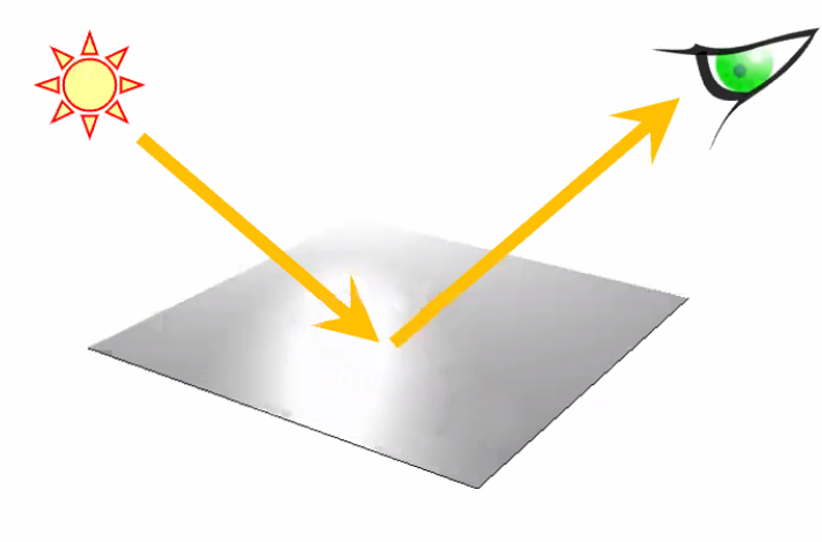
\includegraphics[width=.47\textwidth]{02_grundlagenDerDeflektometrie/spiegelndeOberflaechen/figures/spiegelnd}};
		\node [below=0.2cm of imgGlatt, align=center] {Spiegelnde Oberfläche mit glatter \\ Oberflächenbeschaffenheit};
		\node [anchor=north west] (imgRau) at (0.03\textwidth,0) {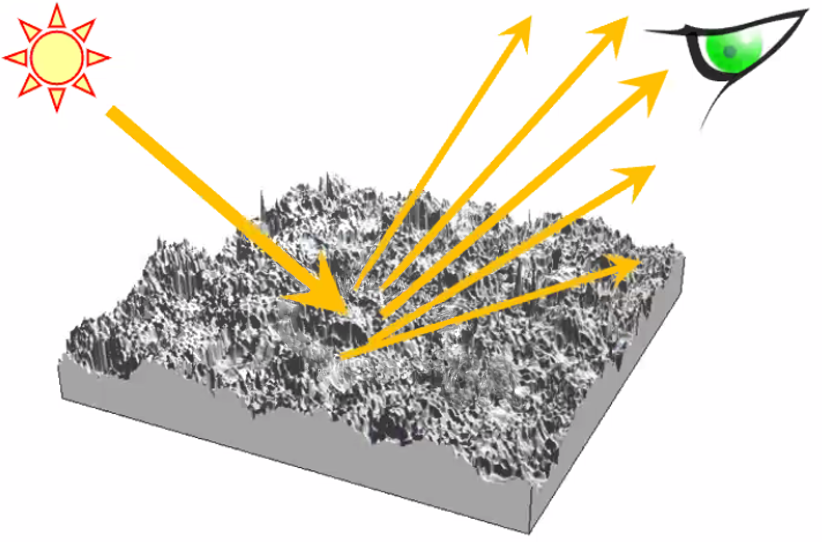
\includegraphics[width=.47\textwidth]{02_grundlagenDerDeflektometrie/spiegelndeOberflaechen/figures/rau}};
		\node [below=0.2cm of imgRau, align=center] {Matte Oberfläche mit rauer \\ Oberflächenbeschaffenheit};
		
	\end{tikzpicture}
\end{adjustbox}
\caption[Spiegelnde und matte Oberflächen]{Spiegelnde bzw. glatte und matte bzw. raue Oberflächen in ihrer mikroskopischen Oberflächenbeschaffenheit. \cite{jenaerOK}}
		\label{tikz:abbGlattUndRau}
	\end{figure}
}
%
\noindent
Durch diese unterschiedlichen Reflexionsarten eignen sich für die Oberflächen unterschiedliche Szenen zur Auswertung der Krümmung.
Während eine spiegelnde Oberfläche ein abbildendes System der Szene darstellt, lässt sich eine Szene über eine matte Oberfläche nicht durch eine Spiegelung beobachten.
Für matte Oberflächen eignet sich daher eine Projektion mit viel Licht zur Beobachtung einer Szene.
Für spiegelnde Oberflächen ist dies aufgrund der hohen Reflexivität ungeeignet.
Stattdessen verwendet man zur Darstellung einer Szene direkt einen Bildschirm (siehe Abbildung  \ref{tikz:abbDeflektometrieVSProjektion}).

% Abbildung: Glatte und Raue Oberfläche
{
	\begin{figure}[H]
		\centering
		\begin{adjustbox}{width=\textwidth}
	\begin{tikzpicture}[every node/.style={inner sep=0,outer sep=0}]
	
		\node [anchor=north east] (imgDeflektometrie) at (-0.03\textwidth,0) {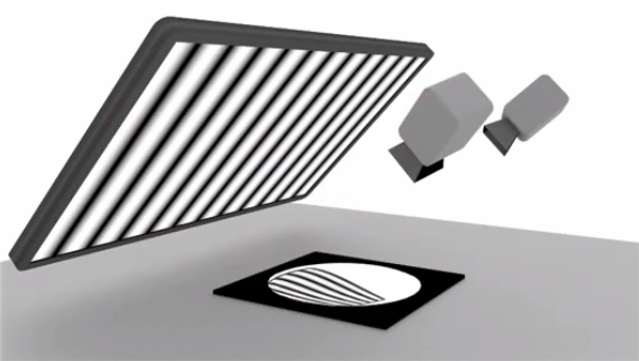
\includegraphics[width=.47\textwidth]{02_grundlagenDerDeflektometrie/spiegelndeOberflaechen/figures/deflektometrie}};
		\node [below=0.2cm of imgDeflektometrie, align=center] {Deflektometrische Verfahren für \\ spiegelnde Oberflächen};
		\node [anchor=north west] (imgProjektion) at (0.03\textwidth,0) {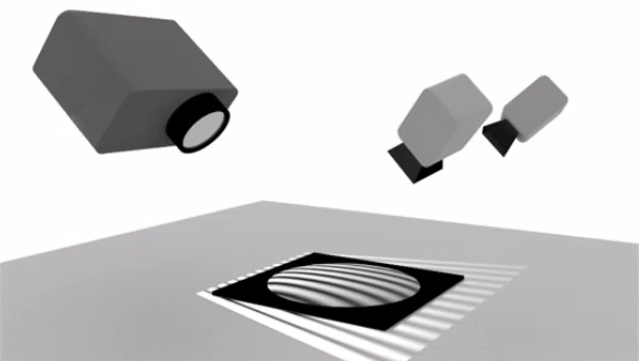
\includegraphics[width=.47\textwidth]{02_grundlagenDerDeflektometrie/spiegelndeOberflaechen/figures/streifenlichtprojektion}};
		\node [below=0.2cm of imgProjektion, align=center] {Streifenlichtprojektion für \\ matte Oberflächen};
		
	\end{tikzpicture}
\end{adjustbox}
\caption[Spiegelnde und matte Oberflächen]{Spiegelnde bzw. glatte und matte bzw. raue Oberflächen in ihrer mikroskopischen Oberflächenbeschaffenheit. \cite{jenaerOK}}
		\label{tikz:abbDeflektometrieVSProjektion}
	\end{figure}
}

\noindent
Im Vergleich erreichen beide Beleuchtungen die Aufnahme einer Szene über der Oberfläche.
Dies ist notwendig, um bestimmte Aussagen über die Oberflächen der Prüfobjekte treffen zu können.
Der wesentliche Unterschied der beiden Verfahren besteht in der Sensitivität gegenüber bestimmten Oberflächenmerkmalen.
Die deflektometrischen Messverfahren sind neigungssensitiv, da die Reflexion direkt von den Oberflächennormalen an den reflektierten Stellen abhängt.
Im Gegensatz dazu ist die Streifenlichtprojektion allein das Hinzufügen einer Projektionslinse, ein höhensensitives Messverfahren für diffus reflektierende Objekte.
Die Oberflächenneigung selbst beeinflusst die aufgenommene Szene bei der Streifenlichtprojektion nicht sehr stark.
Durch die unterschiedliche Funktionsweise der Beleuchtungen für spiegelnde und matte Oberflächen verwendet man auch unterschiedliche Verfahren zur Auswertung der Messungen.
Dennoch wird eine ähnliche Fragestellung behandelt und es lassen sich daher Analogien in den Verfahren feststellen.

\p
Zuletzt ist es noch wichtig, die Besonderheiten von transparenten Objekten zu untersuchen.
Die Oberflächen klarer, transparenter Objekte sind glatt und gehören somit zur Kategorie der spiegelnden Oberflächen.
Entscheidend für die transparente Eigenschaft ist die hohe Lichttransmission solcher Objekte, d. h. die Eigenschaft, das auftreffende Licht durch das Objekt hindurchzulassen.
Das bedeutet, dass das Licht in das Objekt eindringen und innerhalb des Objekts gebrochen und reflektiert werden kann (siehe Abbildung \ref{img:rueckseitenreflex}).

% Abbildung: Rückseitenreflex
\begin{figure}[H]
	\centering
	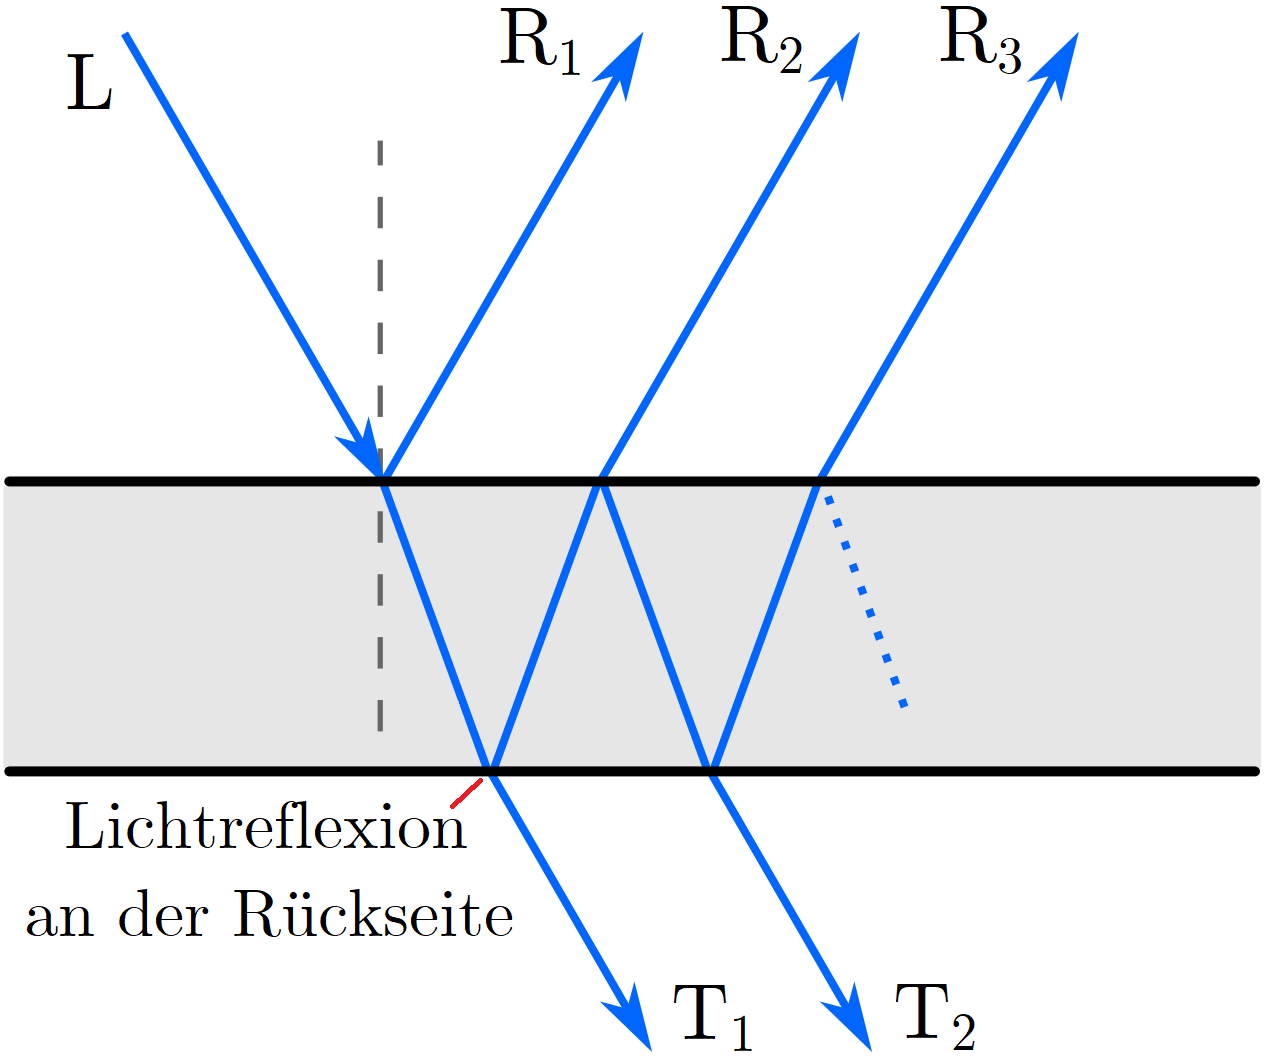
\includegraphics[width=0.4\textwidth]{02_grundlagenDerDeflektometrie/spiegelndeOberflaechen/figures/rueckseitenreflex}
	\caption[Rückseitenreflex]{Brechung und Reflexion an einem ebenen transparenten Objekt. $L$ bezeichnet den auftreffenden Lichtstrahl, $R_i$ die Reflexionen des Lichtstrahls $L$ und $T_i$ die Transmissionen des Lichtstrahls $L$. \cite{deflektometrieScheiben}}
	\label{img:rueckseitenreflex}
\end{figure}

\noindent
Die Lichtreflexion an der Rückseite des Objekts wird Rückseitenreflex genannt.
Dadurch entsteht im Sichtfeld eine Über\-la\-ge\-rung von einer doppelt reflektierten Szene.
Diese Über\-la\-ge\-rung sorgt für Probleme in der Auswertung der aufgenommenen Bilder.
In Abbildung \ref{img:rueckseitenreflexBeispiel} wird der Rückseitenreflex bei einer Glaslinse dargestellt.
Die Szene ist eine Streifenbeleuchtung durch einen Bildschirm.

% Abbildung: Rückseitenreflex Beispiel
\begin{figure}[H]
	\centering
	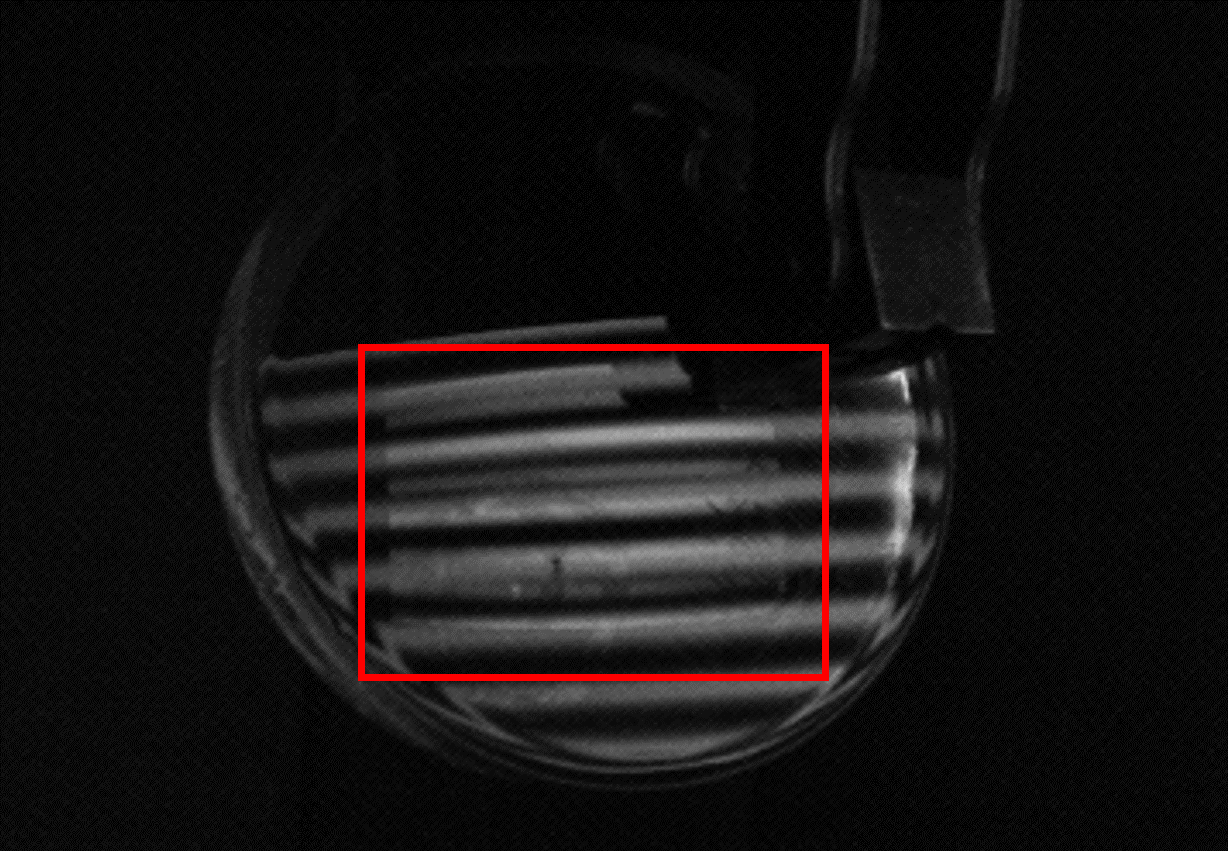
\includegraphics[width=0.5\textwidth]{02_grundlagenDerDeflektometrie/spiegelndeOberflaechen/figures/rueckseitenreflexBeispiel}
	\caption[Beispiel Rückseitenreflex]{Beispiel des Rückseitenreflex an einer transparenten Glaslinse. Im roten Rechteck erkennt man eine leichte zweite Reflexion des Streifenmusters auf dem Bildschirm.}
	\label{img:rueckseitenreflexBeispiel}
\end{figure}

\noindent
Den Effekt des Rückseitenreflexes lässt sich durch bestimmte Verfahren wie z. B. eine undurchsichtige Beschichtung der Oberfläche des transparenten Objekts vermeiden.
Dadurch beschädigt man aber auch die Oberfläche des untersuchten Objekts.
Andere Mög\-lich\-keiten, dies zu reduzieren, sind spezielle Beleuchtungen.
So kann man z. B. statt LCD-Bildschirme Beleuchtungen mit Lichtwellen im ultravioletten Bereich verwenden \cite{invisionUVDeflektometrie}.
Ganz umgehen kann man den Rückseitenreflex, indem man keine Reflexion aufnimmt, sondern mit Durchlicht arbeitet.
Damit kommen allerdings auch Einschränkungen einher, die bestimmte deflektometrische Verfahren ausschließen.

\p
Mit diesem Wissen über den Einsatz bestimmter Beleuchtungsstrategien für spezielle Oberflächen und Objekte kann man Verfahren beschreiben zur Analyse von spiegelnden Oberflächen.